\documentclass[professionalfonts,small]{beamer}
\setbeamercovered{transparent}
\usepackage{psfig}
%\usetheme{boxes}
%\usecolortheme{beaver}
\usepackage{lipsum}% http://ctan.org/pkg/lipsum
\usepackage{setspace}% http://ctan.org/pkg/setspace
\let\oldframetitle\frametitle% Store old \frametitle in \oldframetitle
\renewcommand{\frametitle}[1]{% Redefine \frametitle
  \oldframetitle{#1}\setstretch{1.25}}
%\setstretch{2} <--- uncomment to see the global effect of \setstretch{2}


\newcommand{\Lower}[1]{\smash{\lower 1.5ex \hbox{#1}}}
\newcommand{\STRUT}{\rule{0in}{3ex}}
\begin{document}

\begin{frame}{A Primer on Bond Pricing}

\begin{enumerate}
\item What's a bond?
\item Present value
\item Bond pricing
\item Pricing a call option
\item Back to the government budget constraint
\item The relationship between official interest payments and bond returns
\end{enumerate}

\end{frame}

\begin{frame}{What's a Bond?}

\bigskip

A bond is an I.O.U.  It is a piece of paper that states
``on date $t$, I will pay you $y$ dollars.''

\bigskip

\bigskip

Of course things can be a little more complicated than this.

\end{frame}

\begin{frame}{Non-Coupon and Coupon Bonds}

\begin{enumerate}
\item {\em Non-coupon} or {\em pure discount} bonds state
\begin{quote}
``on (just one) date~$t$ I will pay you $P$
dollars.''
\end{quote}

\item {\em Coupon} bonds promise a stream of payments.

\smallskip

\begin{tabular}{cc}
On date   & I will pay you  \\
 $t_1$      &  $c$ \\
 $t_2$      &  $c$ \\
 $\vdots$   &  $\vdots$ \\
   T        &  $c+P$\\
\end{tabular}
\medskip

``c" stands for {\em coupon}.\\

``P'' stands for {\em principal} or {\em par value} or {\em face value} of the bond.

\end{enumerate}

\end{frame}

\begin{frame}{Present Value}

Is a dollar today and dollar one year (365 days) from now worth the same amount today?
\begin{itemize}
\item Time preference

\item Could take a dollar today, invest it at an interest rate $r$ and have $\$1 \times (1+r)$ in a year.

\item In other words
\begin{eqnarray*}
\mbox{present value}  &=& \frac{\mbox{future value}}{1+r}
\end{eqnarray*}
In this equation $r$ is often referred to as the {\em discount rate}.

\end{itemize}
\end{frame}

\begin{frame}{Present Value (continued)}

If the discount rate is 6 percent, what is a dollar one year from now worth today?
\begin{eqnarray*}
\mbox{present value}  &=& \frac{\$1}{1+.06}  \\
                      &=&  \$0.943 \STRUT
\end{eqnarray*}

\medskip

What is a dollar two years from now worth today?
\begin{eqnarray*}
\mbox{present value}  &=& \frac{1}{1+.06} \times \frac{\$1}{1+.06}  \\
                      &=&  \frac{1}{1+.06} \times \$0.943 \STRUT \\
                      &=&  \$0.890 \STRUT
\end{eqnarray*}



\end{frame}

\begin{frame}{Relationship between bond prices and yields for zero-coupon bonds}

\footnotesize
\begin{itemize}

\item Real, not nominal, variables
\begin{eqnarray*}
q_{t,t+j} &=& \mbox{real price of one unit of time $t+j$ consumption}\\
          &&  \mbox{at time t}\\
r_{t,t+j} &=& \mbox{yield of a $j$-period $t+j$ pure discount}\\
           && \mbox{(zero coupon) bond at time t} \\
q_{t,t+j} &=& \exp(-j r_{t,t+j}) \approx \frac{1}{(1+r_{t,t+j})^j} \STRUT
\end{eqnarray*}

\item Take logs of both sides
\begin{eqnarray*}
\log q_{t,t+j} &=& -j r_{t,t+j} \\
r_{t,t+j} &=& - \frac{\log q_{t,t+j}}{j}
\end{eqnarray*}

\end{itemize}

\end{frame}

\begin{frame}{Handy Math Fact}
\footnotesize

\begin{itemize}

\item $\log (1+ r_{t,t+j}) \approx r_{t,t+j}$ for ``small'' $r_{t,t+j}$'s

\medskip

\item Why?  Taylor Series (Newton)
\begin{eqnarray*}
f(x) &=& \log(1+x)\\
     &\approx& f(x_0) + (x-x_0)f'(x_0) |_{x=x_0}
\end{eqnarray*}

\medskip

\item Apply with $f(x) = \log(1+x)$ and $x_0 = 0$, then
\begin{eqnarray*}
\log(1+x) &\approx& 0 + x\left(\frac{1}{1+x}\right) |_{x=x_0} \\
          &\approx& x
\end{eqnarray*}

\end{itemize}

\end{frame}

\begin{frame}{Happy Meal Theorem of Bond Pricing}

\begin{itemize}

\item Happy meal: burger, fries, drink, toy

\medskip

\item Consider a bond that at time $t$ promises to pay
\begin{center}
\begin{tabular}{cccccc}
  $t$    &   $t+1$   &  $t+2$  &  $t+3$   & ...  & $t+T$  \\
\hline
   0      &    $c$    &   $c$   &   $c$    &  ... & $P+c$   \\
\end{tabular}
\end{center}

\medskip

\item The value of the bond at time $t$ is then
\begin{eqnarray*}
V_t &=& c q_{t,t+1} + c q_{t,t+2} +  ... + c q_{t,t+T} + P q_{t,t+T} \\
    &=& c (q_{t,t+1} + q_{t,t+2} +  ... + q_{t,t+T}) + P q_{t,t+T}
\end{eqnarray*}

\end{itemize}

\end{frame}

\begin{frame}{Happy Meal Theorem of Bond Pricing (con't)}

\begin{itemize}

\item The value of this same bond at $t+1$, after $c$ has been paid, is
\begin{eqnarray*}
V_{t+1}  = c (q_{t+1,t+2} + q_{t+1,t+3} +  ... + q_{t+1,t+T}) + P q_{t+1,t+T}
\end{eqnarray*}

\medskip

\item Evidently
\begin{eqnarray*}
V_t = q_{t,t+1} \left( c + V_{t+1} \right)
\end{eqnarray*}

\end{itemize}

\end{frame}

\begin{frame}{Forward Rates}
\footnotesize

\begin{itemize}

\item With no uncertainty, the law of one price asserts that
\begin{eqnarray*}
q_{t,t+j} = q_{t,t+1} q_{t+1,t+j}
\end{eqnarray*}

\medskip

\item Two ways at time $t$ to buy one unit of consumption at $t+j$
\begin{enumerate}
\footnotesize
\item either pay $q_{t,t+j}$ at time $t$, or
\item pay $q_{t,t+1}$ at time $t$ and $q_{t+1,t+j}$ at time $t+1$
\end{enumerate}

\medskip

\item Define
\begin{eqnarray*}
\tilde{q}^t_{t+1,t+j} \equiv \frac{q_{t,t+j}}{q_{t,t+1}}
\end{eqnarray*}
as the {\em forward price} at $t$


\item With no uncertainty about future interest rates
\begin{eqnarray*}
\tilde{q}^t_{t+1,t+j} = q_{t+1,t+j}
\end{eqnarray*}


\item When there is uncertainty, these two won't necessarily be equal.

\end{itemize}

\end{frame}

\begin{frame}{Yield to Maturity}

\begin{itemize}

\item The yield to maturity is the unique $r$ that satisfies
\begin{eqnarray*}
V = \frac{c}{1+r}  + \frac{c}{(1+r)^2} + \frac{c}{(1+r)^3} + ... + \frac{c+P}{(1+r)^T}
\end{eqnarray*}

given $V$, $c$, $P$, and $T$.

\bigskip

\item Usually can not be solved for by hand.

\bigskip

\item It is sometimes just called the yield.

\end{itemize}

\end{frame}


\begin{frame}{Three Period Coupon Bond Example}
\footnotesize

\begin{itemize}

\item Bond issued at $t=0$ and is a riskless claim on stream
\begin{center}
\begin{tabular}{ccc}
  $0$    &   $1$   &  $2$   \\
\hline
   0     &   $c$   &   $c+P$  \\
\end{tabular}
\end{center}
Again, $c$ is the coupon and $P$ is the principal or par value

\medskip

\item The time $t=0$ price of the bond is
\begin{eqnarray*}
V_0 = q_{0,1} c + q_{0,2}(c+P)
\end{eqnarray*}

\medskip

\item After payment of the coupon, the price of the bond at time $t=1$ is
\begin{eqnarray*}
V_1 = q_{1,2}(c+P)
\end{eqnarray*}

\end{itemize}

\end{frame}

\begin{frame}{Value of a Call Option}

\footnotesize

\begin{itemize}

\item At $t=0$, you purchase the right to buy the bond at $t=1$ at a price $P$.
\begin{itemize}
\item thus, $P$ serves as both the {\em par value} and the {\em strike price}.
\end{itemize}

\medskip

\item The value of this option at time 1 is
\begin{eqnarray*}
\max(0,V_1 - P)
\end{eqnarray*}

\medskip

\item You will want to exercise the call option is
\begin{eqnarray*}
P <  V_1 = q_{1,2}(c+P)
\end{eqnarray*}

\end{itemize}

\end{frame}

\begin{frame}{Three Period Coupon Bond Example (con't)}

\footnotesize

\begin{itemize}

\item An interesting benchmark case: when is $V_1 = P$?

Solve equation
\begin{eqnarray*}
V_1 = P = q_{1,2}(c+P)
\end{eqnarray*}
for $q_{1,2}$

That is:
\begin{eqnarray*}
q_{1,2} = \frac{P}{c+P}
\end{eqnarray*}
or
\begin{eqnarray*}
1+r_{1,2} \approx \frac{c+P}{P}
\end{eqnarray*}

\item Question:  when is $V_0 = V_1 = P$?

\item Often see that Congress is reluctant to issue bonds selling at less than $P$.

\end{itemize}

\end{frame}

\begin{frame}{Extend the Example: Interest rate risk}

\begin{itemize}

\item payouts known for certain

\medskip

\item uncertain future interest rates

\medskip

\item three time periods: $0$, $1$, and $2$.
\begin{eqnarray*}
q_{0,1}, \; \; q_{1,2}(H), \; \; q_{1,2}(L) \; \; \mbox{ where $q_{1,2}(H) > q_{1,2}(L)$}
\end{eqnarray*}

\medskip


\item Assume $q_{1,2}(H)$ occurs with probability $\pi_0$\\
And $q_{1,2}(L)$ occurs with probability $1-\pi_0$

\end{itemize}

\end{frame}

\begin{frame}{Extend the Example: Interest rate risk (con't)}

\begin{itemize}
\footnotesize

\item Simple ``expectations theory" of the term structure
\begin{eqnarray*}
q_{0,2} &=& q_{0,1}(\pi_0 q_{1,2}(H) + (1-\pi_0) q_{1,2}(L)) \\
\frac{q_{0,2}}{q_{0,1}} &\equiv& \tilde{q}^0_{1,2} = \pi_0 q_{1,2}(H) + (1-\pi_0) q_{1,2}(L)
\end{eqnarray*}

\item $\tilde{q}^0_{1,2}$ is the {\em forward price}.
\begin{itemize}
\footnotesize
\item is an average of the two possible prices next period
\item no adjustment for risk
\item fancier theories adjust for risk
\item whose $\pi_0$? (rational expectations)
\end{itemize}

\item Similarly
\begin{eqnarray*}
\tilde{r}^0_{1,2} = \pi_0 r_{1,2}(L) + (1-\pi_0) r_{1,2}(H)
\end{eqnarray*}
flip the $H$ and $L$ because high bond prices mean low interest rates

\end{itemize}

\end{frame}

\begin{frame}{Value of a Call Option}

\footnotesize
\begin{itemize}

\item At $t=0$, you purchase the right to buy the bond at $t=1$ at a price $P$.

\item Assume that
\begin{eqnarray*}
q_{1,2}(H) > q_{1,2}(L)
\end{eqnarray*}
and
\begin{eqnarray*}
q_{1,2}(H)(c+P) > P > q_{1,2}(L)(c+P)
\end{eqnarray*}

\item If state H occurs the time $1$ value of the call is
\begin{eqnarray*}
V_1^{call} = \max(0,q_{1,2}(H)(c+P) -P) > 0
\end{eqnarray*}

\item If state L occurs the time $1$ value of the call is
\begin{eqnarray*}
V_1^{call} = \max(0, q_{1,2}(L)(c+P) -P) = 0
\end{eqnarray*}

\item Therefore, the time $0$ value of the call is
\begin{eqnarray*}
V_0^{call} = q_{0,1} \left[ \pi_0(q_{1,2}(H)(c+P) -P) \right]
\end{eqnarray*}

\end{itemize}

\end{frame}

%  Tom, I am going to leave this case for a problem set problem.
%
%\begin{frame}
%
%\begin{itemize}
%
%\item Example: With constant interest rates satisfying the ``Congress wishful thinking condition"
%\begin{eqnarray*}
%P = q_{t,t+1}(c+P)
%\end{eqnarray*}
%or
%\begin{eqnarray*}
%q_{t,t+1} = \frac{P}{c+P} \; \mbox{ for all $t$}
%\end{eqnarray*}
%then the value of the call is zero.

%\item Hence
%\begin{eqnarray*}
%q_{1,2}(H) = q_{1,2}(L) = \frac{P}{P+c}
%\end{eqnarray*}
%
%\end{itemize}
%
%\end{frame}

\begin{frame}{Pricing a Callable Bond}
\footnotesize

\begin{itemize}

\item Consider
\begin{eqnarray*}
q_{1,2}(H)  > \frac{P}{P+c} > q_{1,2}(L)
\end{eqnarray*}

\item Value of a non-callable bond
\begin{eqnarray*}
V_0 = q_{0,1} c + q_{0,2}(c+P)
\end{eqnarray*}

\item Suppose the government issues a two period bond that is callable in period 1 at par.

\item A callable bond can be decomposed into two parts
\begin{enumerate}
\footnotesize
\item non-callable bond
\item call option
\end{enumerate}

\item When the government issues a callable bond, it sells part 1 and buys part 2.

\item Happy Meal Theorem:  Value of a callable bond
\begin{eqnarray*}
V_0 - V_0^{call}
\end{eqnarray*}

\end{itemize}

\end{frame}

\begin{frame}{Example: 20 Year Coupon Bond}

Suppose that this year (January 1, 2013) you invest in a 6\% percent 2033 U.S. Treasury bond with a
face value of \$100.

\begin{center}
\begin{tabular}{ccccccc}
  2013    &   2014   &  2015  &  2016   & ...  & 2032  & 2033\\
\hline
   0      &    6    &   6   &   6    &  ... & 6    & 106 \\
\hline
\end{tabular}
\end{center}

\end{frame}

\begin{frame}{Example: 20 Year Coupon Bond}
\footnotesize

\begin{itemize}

\item No uncertainty

\medskip

\item Apply the Happy Meal Theorem
\begin{eqnarray*}
V_{2013} &=& q_{2013,2014} C + q_{2013,2015} C + q_{2013,2016} C +  \\
    && ... + q_{2013,2033} ( C + P)
\end{eqnarray*}

\medskip

\item Assume a constant interest rate
\begin{itemize}

\footnotesize

\item a flat term structure

\smallskip

\item $r_{2013,2014}$ = $r_{2014,2015}$ = $r_{2015,2016}$ = $r_{2016,2017} ... = \bar{r} $

\smallskip


\item So $\bar{r}$ is the yield-to-maturity or YTM.
\end{itemize}

\end{itemize}

\end{frame}

\begin{frame}{Use Excel to do the valuations}

\begin{itemize}

\item Let EXCEL do the calculations for us
\begin{itemize}
\item Set $\bar{r}=.06$

\item Set $\bar{r}=.03$

\item Set $\bar{r} =.09$
\end{itemize}

\medskip

\item If a bond's coupon rate is
\begin{itemize}
\item less than its YTM, then the bond is selling at a {\em discount}.
\item more than its YTM, then the bond is selling at a {\em premium}.
\item equal to its YTM, then the bond is selling at {\em par}.
\end{itemize}

\end{itemize}

\end{frame}

\begin{frame}{One Type of Risk:  Interest Rate Risk}

\begin{itemize}

\item Suppose that the (constant) interest rate is 6 percent

\medskip

\item Five years from now, in 2018, (after we receive the 2018 coupon payment), there is
\begin{itemize}
\item $\pi$ chance the interest rate will fall to 3\% from 2018 on
\item $1-\pi$ chance the interest rate will rise to 9\% from 2018 on
\end{itemize}

\medskip

\item How does this risk affect our bond pricing?
\begin{itemize}
\item Assumption:  we are risk-neutral.
\item We need to price both possibilities.
\end{itemize}

\end{itemize}

\end{frame}

\begin{frame}{Work Backwards}
\footnotesize


What is our 20 year, \$100 face value, 6\% coupon, bond worth in 2018?

\begin{itemize}
\item CASE I:  Interest rate falls to 3 percent
\begin{eqnarray*}
V_{2018}^{.03} = \sum_{t=1}^{15}\frac{C}{(1+0.03)^t} + \frac{P}{(1+.03)^{15}}
\end{eqnarray*}
\item  CASE II: Interest rate rises to 9 percent
\begin{eqnarray*}
V_{2018}^{.09} = \sum_{t=1}^{15}\frac{C}{(1+0.09)^t} + \frac{P}{(1+.09)^{15}}
\end{eqnarray*}

\item So what is our bond worth today in 2013?
\begin{eqnarray*}
V_{2013} =  \sum_{t=1}^{5}\frac{C}{(1+0.06)^t} + \pi \frac{V_{2018}^{.03}}{(1+.06)^5} + (1-\pi) \frac{V_{2018}^{.09}}{(1+.06)^5}
\end{eqnarray*}

\end{itemize}

\end{frame}

\begin{frame}{A Call Option}

\footnotesize

Consider the following contract: Today (in 2013) I sell you the right to purchase this bond in year 2018 for \$100.
You don't have to purchase the bond.  It is an option.

\bigskip
How much is this option worth?
\begin{itemize}
\item Again, work backwards.  In 2018, consider both cases
\begin{enumerate}
\item CASE I:  $ \max(0, V_{2018}^{.03} - 100) $
\item CASE II: $ \max(0, V_{2018}^{.09} - 100) $
\end{enumerate}

\item In 2018
\begin{eqnarray*}
V_{2018}^{call} = \pi \max(0, V_{2018}^{.03} - 100) + (1-\pi) \max(0, V_{2018}^{.09} - 100)
\end{eqnarray*}

\item In 2013
\begin{eqnarray*}
V_{2013}^{call}  = \frac{V_{2018}^{call}}{(1+.06)^5}
\end{eqnarray*}

\end{itemize}
\end{frame}

\begin{frame}{What's the price of a 5-20 bond?}

\begin{itemize}

\item Consider a 20 year coupon bond that callable at par by the Treasury after five year.

\medskip

\item Happy Meal Theorem
\begin{eqnarray*}
V_{2013} - V_{2013}^{call}
\end{eqnarray*}

\medskip

\item If a callable bond always sells for less than a non-callable bond, why would a government ever issue a callable bond?

\end{itemize}

\end{frame}



\begin{frame}{Using the G. B. C. to Price Government Debt}
\medskip

\begin{itemize}

\item The price of a bond is the discounted present value of the stream of promised payments

\medskip

\item We could think of the government budget constraint much the same way.  Recall we can rewrite the g.b.c. as:
\begin{eqnarray*}
B_{t}  &=&   \sum_{j=1}^{\infty} \left(\frac{1}{1+r}\right)^{j}(T_{t+j} - G_{t+j})
\end{eqnarray*}

\medskip

\item Last lecture, we assumed the future paths of $T$ and $G$ will have to
adjust to satisfy the current value of $B_t$.

\end{itemize}
\end{frame}

\begin{frame}
\begin{itemize}

\item But what if the expected value of
\begin{eqnarray*}
\sum_{j=1}^{\infty} \left(\frac{1}{1+r}\right)^{j}(T_{t+j} - G_{t+j})
\end{eqnarray*}
 is less than the face value of the current stock of debt?
\begin{itemize}
\item If future $T$s and $G$s are constrained, bond prices will adjust
\end{itemize}

\bigskip

\item So is the government budget constraint a constraint?  Or is it a pricing formula?

\end{itemize}
\end{frame}

\begin{frame}{Bond Returns}

\begin{itemize}

\item Suppose you buy a bond at period $t$ a price $V_t$, hold it one period, and sell it at price $V_{t+1}$.  What is your return?

\item In period $t+1$ you receive the coupon payment and the sales price.

\item So the one-period ex-post holding return for a bond is
\begin{eqnarray*}
1+r_{t,t+1} = \frac{C + V_{t+1}}{V_t}
\end{eqnarray*}

\end{itemize}

\end{frame}

\begin{frame}{Recorded Government Interest Payments}

\footnotesize

\begin{itemize}

\item What the Bureau of the Public Debt reports as its nominal interest payments
\begin{itemize}
\item discount the bills
\item add up the coupons on notes and bonds
\end{itemize}\medskip

\medskip

\item Answers the question ``how many dollars must
the Treasury devote to paying coupons on this period's outstanding
government bonds while rolling over the nominal stock of treasury
bills?''  \medskip

\medskip

\item Leaves out capital gains and losses on Treasury notes and bonds
obligations.

\medskip

\item Does not answer the question:  what return did government bond holders receive?

\end{itemize}
\end{frame}

\begin{frame}
\centerline{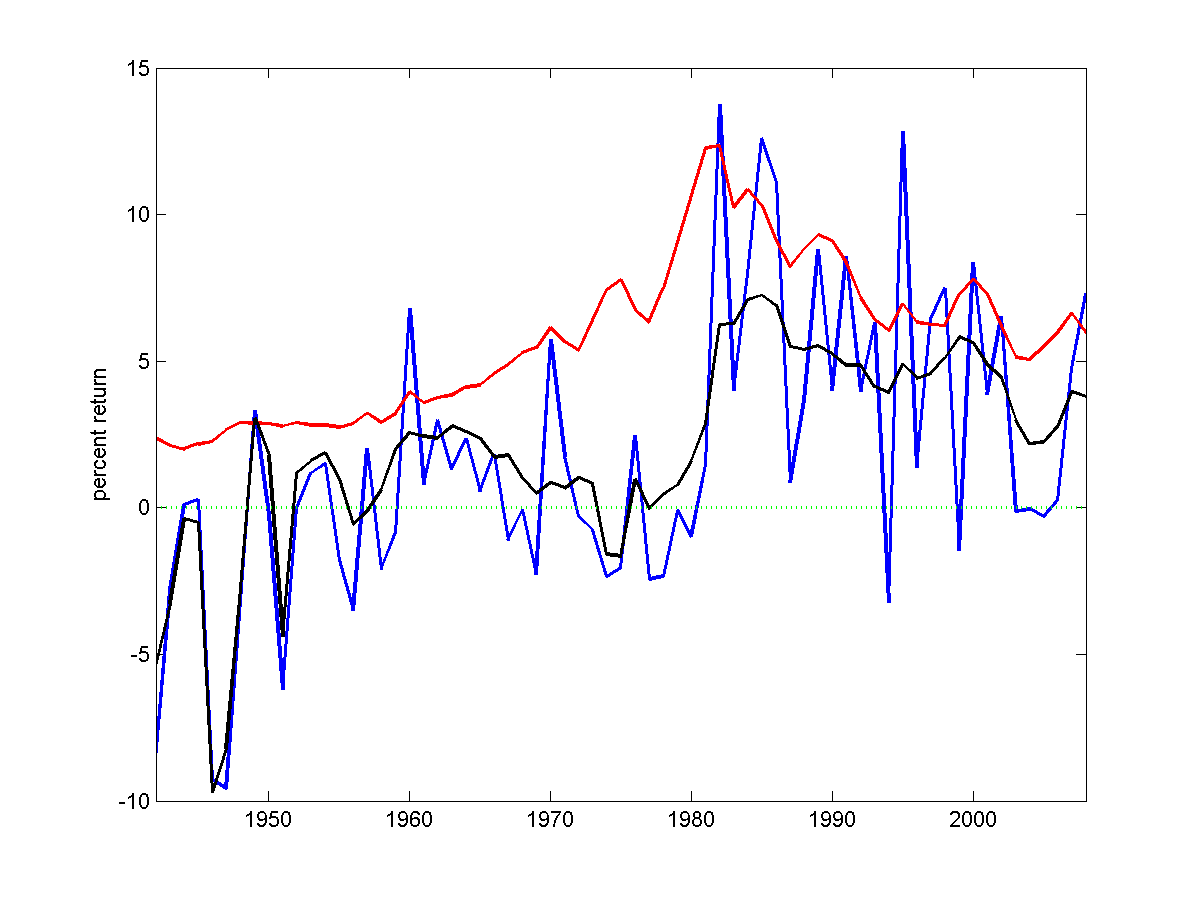
\psfig{file=cof_returns_gdpdef.ps,width=3.8in}}
\vspace{.1in}
\centerline{Comparison Between Official Interest Payments and Returns to Bondholders}
\end{frame}



\begin{frame}{Means and Standard Deviations of Returns}

\begin{center}
\begin{tabular}{lcc}
Variable                          &  Mean    & Std Dev \\
\hline
Official Interest/Debt               &   5.20   &    2.54 \\
Inflation                            &   3.73   &    2.67 \\
Official Interest/Debt - inflation   &   1.47   &    3.31 \\
Real Return on Marketable Debt       &   1.63   &    4.86 \\
\end{tabular}
\end{center}

\end{frame}

\begin{frame}{Does this Accounting Issue Matter?}
\footnotesize
\begin{itemize}

\item Reported interest payments on the debt are not the $R_t B^G_{t}$ in the government budget constraint.
Is this a big deal?

\medskip

\item The Treasury
\begin{enumerate}
\footnotesize
\item reports the par value rather than the market value of its debt, and
\item typically sets the coupon rate so that at auction, bonds sell near par.
\end{enumerate}

\medskip

\item In this case the ytm equals the coupon rate, and the par value and the market value will not be that different.

\end{itemize}
\end{frame}
\begin{frame}

\begin{itemize}

\item Will get big differences between the par value and market value when there are large capital gains and losses (perhaps due to changes in inflation)
\begin{itemize}
\item War of 1812
\end{itemize}

\bigskip

\item Talk these days about using inflation to erode the debt. To frame the tradeoff, need to properly account for interest the government actually pays.

\end{itemize}

\end{frame}

\end{document}

